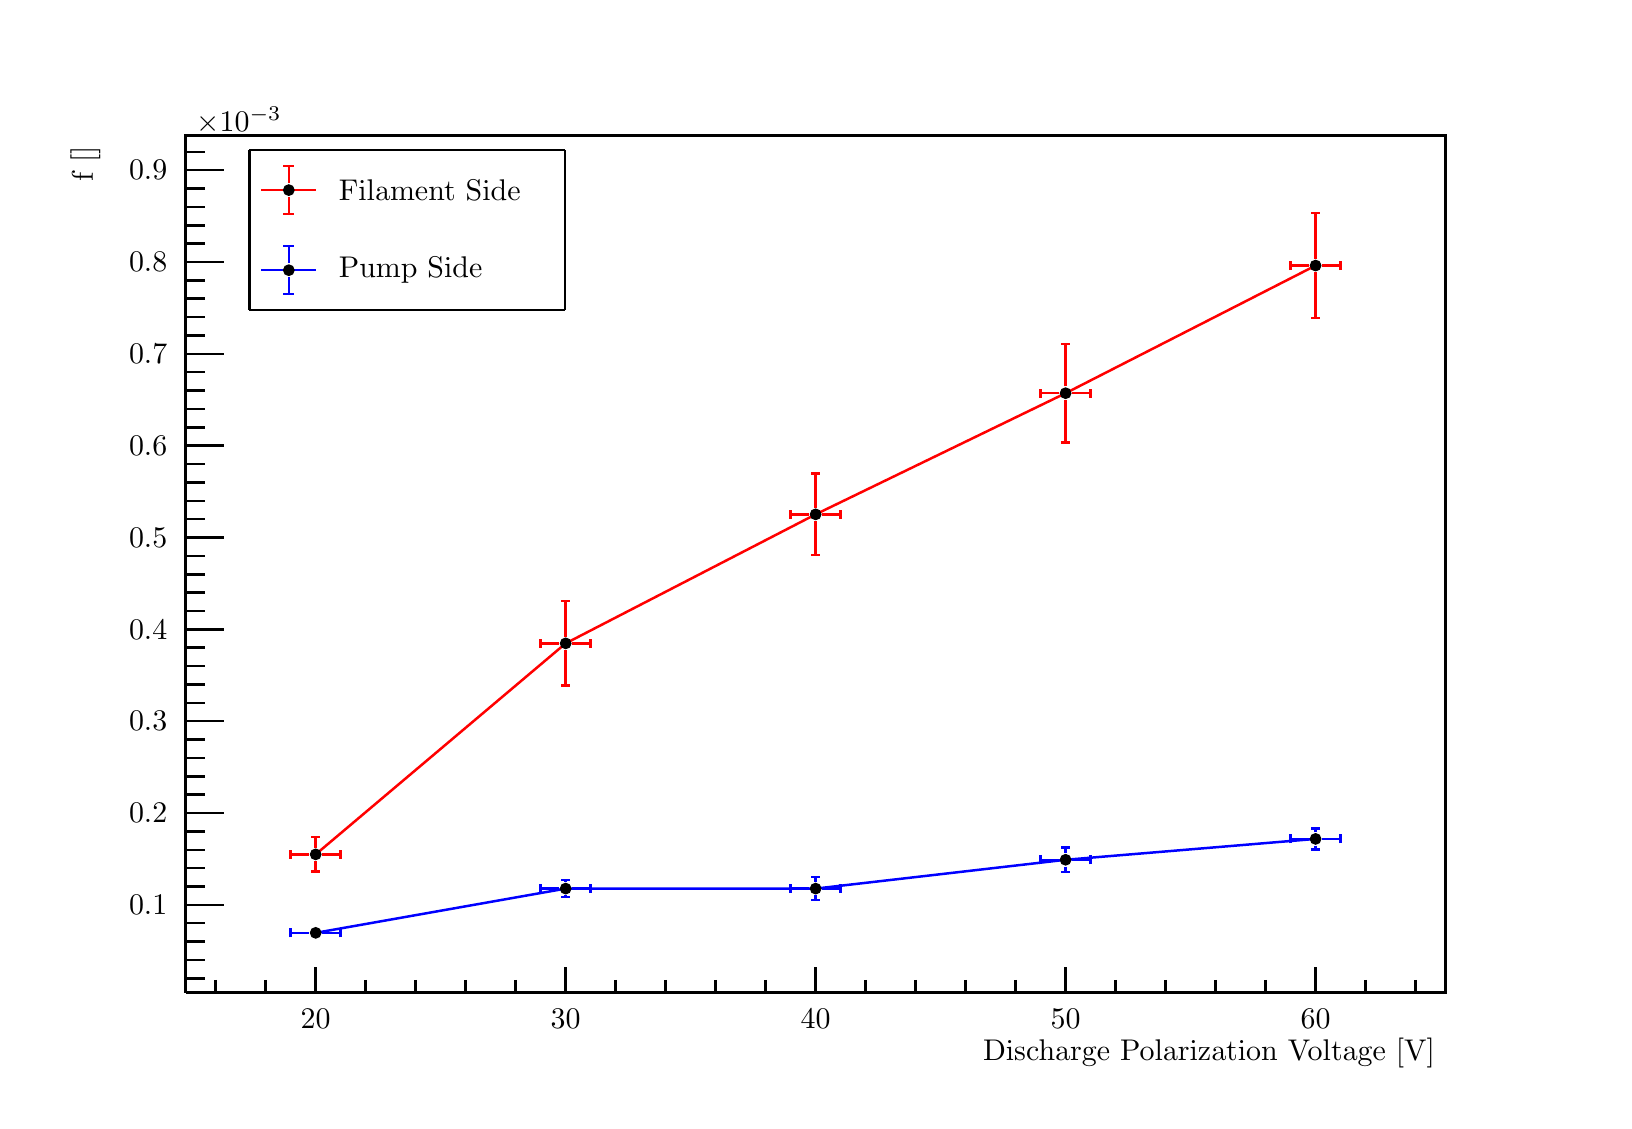
\begin{tikzpicture}
\pgfdeclareplotmark{cross} {
\pgfpathmoveto{\pgfpoint{-0.3\pgfplotmarksize}{\pgfplotmarksize}}
\pgfpathlineto{\pgfpoint{+0.3\pgfplotmarksize}{\pgfplotmarksize}}
\pgfpathlineto{\pgfpoint{+0.3\pgfplotmarksize}{0.3\pgfplotmarksize}}
\pgfpathlineto{\pgfpoint{+1\pgfplotmarksize}{0.3\pgfplotmarksize}}
\pgfpathlineto{\pgfpoint{+1\pgfplotmarksize}{-0.3\pgfplotmarksize}}
\pgfpathlineto{\pgfpoint{+0.3\pgfplotmarksize}{-0.3\pgfplotmarksize}}
\pgfpathlineto{\pgfpoint{+0.3\pgfplotmarksize}{-1.\pgfplotmarksize}}
\pgfpathlineto{\pgfpoint{-0.3\pgfplotmarksize}{-1.\pgfplotmarksize}}
\pgfpathlineto{\pgfpoint{-0.3\pgfplotmarksize}{-0.3\pgfplotmarksize}}
\pgfpathlineto{\pgfpoint{-1.\pgfplotmarksize}{-0.3\pgfplotmarksize}}
\pgfpathlineto{\pgfpoint{-1.\pgfplotmarksize}{0.3\pgfplotmarksize}}
\pgfpathlineto{\pgfpoint{-0.3\pgfplotmarksize}{0.3\pgfplotmarksize}}
\pgfpathclose
\pgfusepathqstroke
}
\pgfdeclareplotmark{cross*} {
\pgfpathmoveto{\pgfpoint{-0.3\pgfplotmarksize}{\pgfplotmarksize}}
\pgfpathlineto{\pgfpoint{+0.3\pgfplotmarksize}{\pgfplotmarksize}}
\pgfpathlineto{\pgfpoint{+0.3\pgfplotmarksize}{0.3\pgfplotmarksize}}
\pgfpathlineto{\pgfpoint{+1\pgfplotmarksize}{0.3\pgfplotmarksize}}
\pgfpathlineto{\pgfpoint{+1\pgfplotmarksize}{-0.3\pgfplotmarksize}}
\pgfpathlineto{\pgfpoint{+0.3\pgfplotmarksize}{-0.3\pgfplotmarksize}}
\pgfpathlineto{\pgfpoint{+0.3\pgfplotmarksize}{-1.\pgfplotmarksize}}
\pgfpathlineto{\pgfpoint{-0.3\pgfplotmarksize}{-1.\pgfplotmarksize}}
\pgfpathlineto{\pgfpoint{-0.3\pgfplotmarksize}{-0.3\pgfplotmarksize}}
\pgfpathlineto{\pgfpoint{-1.\pgfplotmarksize}{-0.3\pgfplotmarksize}}
\pgfpathlineto{\pgfpoint{-1.\pgfplotmarksize}{0.3\pgfplotmarksize}}
\pgfpathlineto{\pgfpoint{-0.3\pgfplotmarksize}{0.3\pgfplotmarksize}}
\pgfpathclose
\pgfusepathqfillstroke
}
\pgfdeclareplotmark{newstar} {
\pgfpathmoveto{\pgfqpoint{0pt}{\pgfplotmarksize}}
\pgfpathlineto{\pgfqpointpolar{44}{0.5\pgfplotmarksize}}
\pgfpathlineto{\pgfqpointpolar{18}{\pgfplotmarksize}}
\pgfpathlineto{\pgfqpointpolar{-20}{0.5\pgfplotmarksize}}
\pgfpathlineto{\pgfqpointpolar{-54}{\pgfplotmarksize}}
\pgfpathlineto{\pgfqpointpolar{-90}{0.5\pgfplotmarksize}}
\pgfpathlineto{\pgfqpointpolar{234}{\pgfplotmarksize}}
\pgfpathlineto{\pgfqpointpolar{198}{0.5\pgfplotmarksize}}
\pgfpathlineto{\pgfqpointpolar{162}{\pgfplotmarksize}}
\pgfpathlineto{\pgfqpointpolar{134}{0.5\pgfplotmarksize}}
\pgfpathclose
\pgfusepathqstroke
}
\pgfdeclareplotmark{newstar*} {
\pgfpathmoveto{\pgfqpoint{0pt}{\pgfplotmarksize}}
\pgfpathlineto{\pgfqpointpolar{44}{0.5\pgfplotmarksize}}
\pgfpathlineto{\pgfqpointpolar{18}{\pgfplotmarksize}}
\pgfpathlineto{\pgfqpointpolar{-20}{0.5\pgfplotmarksize}}
\pgfpathlineto{\pgfqpointpolar{-54}{\pgfplotmarksize}}
\pgfpathlineto{\pgfqpointpolar{-90}{0.5\pgfplotmarksize}}
\pgfpathlineto{\pgfqpointpolar{234}{\pgfplotmarksize}}
\pgfpathlineto{\pgfqpointpolar{198}{0.5\pgfplotmarksize}}
\pgfpathlineto{\pgfqpointpolar{162}{\pgfplotmarksize}}
\pgfpathlineto{\pgfqpointpolar{134}{0.5\pgfplotmarksize}}
\pgfpathclose
\pgfusepathqfillstroke
}
\definecolor{c}{rgb}{1,1,1};
\draw [color=c, fill=c] (0,0) rectangle (20,13.6103);
\draw [color=c, fill=c] (2,1.36103) rectangle (18,12.2493);
\definecolor{c}{rgb}{0,0,0};
\draw [c,line width=0.9] (2,1.36103) -- (2,12.2493) -- (18,12.2493) -- (18,1.36103) -- (2,1.36103);
\definecolor{c}{rgb}{1,1,1};
\draw [color=c, fill=c] (2,1.36103) rectangle (18,12.2493);
\definecolor{c}{rgb}{0,0,0};
\draw [c,line width=0.9] (2,1.36103) -- (2,12.2493) -- (18,12.2493) -- (18,1.36103) -- (2,1.36103);
\draw [c,line width=0.9] (2,1.36103) -- (18,1.36103);
\draw [c,line width=0.9] (3.65079,1.68768) -- (3.65079,1.36103);
\draw [c,line width=0.9] (4.28571,1.52436) -- (4.28571,1.36103);
\draw [c,line width=0.9] (4.92064,1.52436) -- (4.92064,1.36103);
\draw [c,line width=0.9] (5.55556,1.52436) -- (5.55556,1.36103);
\draw [c,line width=0.9] (6.19048,1.52436) -- (6.19048,1.36103);
\draw [c,line width=0.9] (6.8254,1.68768) -- (6.8254,1.36103);
\draw [c,line width=0.9] (7.46032,1.52436) -- (7.46032,1.36103);
\draw [c,line width=0.9] (8.09524,1.52436) -- (8.09524,1.36103);
\draw [c,line width=0.9] (8.73016,1.52436) -- (8.73016,1.36103);
\draw [c,line width=0.9] (9.36508,1.52436) -- (9.36508,1.36103);
\draw [c,line width=0.9] (10,1.68768) -- (10,1.36103);
\draw [c,line width=0.9] (10.6349,1.52436) -- (10.6349,1.36103);
\draw [c,line width=0.9] (11.2698,1.52436) -- (11.2698,1.36103);
\draw [c,line width=0.9] (11.9048,1.52436) -- (11.9048,1.36103);
\draw [c,line width=0.9] (12.5397,1.52436) -- (12.5397,1.36103);
\draw [c,line width=0.9] (13.1746,1.68768) -- (13.1746,1.36103);
\draw [c,line width=0.9] (13.8095,1.52436) -- (13.8095,1.36103);
\draw [c,line width=0.9] (14.4444,1.52436) -- (14.4444,1.36103);
\draw [c,line width=0.9] (15.0794,1.52436) -- (15.0794,1.36103);
\draw [c,line width=0.9] (15.7143,1.52436) -- (15.7143,1.36103);
\draw [c,line width=0.9] (16.3492,1.68768) -- (16.3492,1.36103);
\draw [c,line width=0.9] (3.65079,1.68768) -- (3.65079,1.36103);
\draw [c,line width=0.9] (3.01587,1.52436) -- (3.01587,1.36103);
\draw [c,line width=0.9] (2.38095,1.52436) -- (2.38095,1.36103);
\draw [c,line width=0.9] (16.3492,1.68768) -- (16.3492,1.36103);
\draw [c,line width=0.9] (16.9841,1.52436) -- (16.9841,1.36103);
\draw [c,line width=0.9] (17.619,1.52436) -- (17.619,1.36103);
\draw [anchor=base] (3.65079,0.911891) node[scale=1.08185, color=c, rotate=0]{20};
\draw [anchor=base] (6.8254,0.911891) node[scale=1.08185, color=c, rotate=0]{30};
\draw [anchor=base] (10,0.911891) node[scale=1.08185, color=c, rotate=0]{40};
\draw [anchor=base] (13.1746,0.911891) node[scale=1.08185, color=c, rotate=0]{50};
\draw [anchor=base] (16.3492,0.911891) node[scale=1.08185, color=c, rotate=0]{60};
\draw [anchor= east] (18,0.598854) node[scale=1.08185, color=c, rotate=0]{Discharge Polarization Voltage [V]};
\draw [c,line width=0.9] (2,1.36103) -- (2,12.2493);
\draw [c,line width=0.9] (2.48,2.47673) -- (2,2.47673);
\draw [c,line width=0.9] (2.24,2.71) -- (2,2.71);
\draw [c,line width=0.9] (2.24,2.94327) -- (2,2.94327);
\draw [c,line width=0.9] (2.24,3.17654) -- (2,3.17654);
\draw [c,line width=0.9] (2.24,3.40981) -- (2,3.40981);
\draw [c,line width=0.9] (2.48,3.64308) -- (2,3.64308);
\draw [c,line width=0.9] (2.24,3.87635) -- (2,3.87635);
\draw [c,line width=0.9] (2.24,4.10962) -- (2,4.10962);
\draw [c,line width=0.9] (2.24,4.34289) -- (2,4.34289);
\draw [c,line width=0.9] (2.24,4.57617) -- (2,4.57617);
\draw [c,line width=0.9] (2.48,4.80944) -- (2,4.80944);
\draw [c,line width=0.9] (2.24,5.04271) -- (2,5.04271);
\draw [c,line width=0.9] (2.24,5.27598) -- (2,5.27598);
\draw [c,line width=0.9] (2.24,5.50925) -- (2,5.50925);
\draw [c,line width=0.9] (2.24,5.74252) -- (2,5.74252);
\draw [c,line width=0.9] (2.48,5.97579) -- (2,5.97579);
\draw [c,line width=0.9] (2.24,6.20906) -- (2,6.20906);
\draw [c,line width=0.9] (2.24,6.44233) -- (2,6.44233);
\draw [c,line width=0.9] (2.24,6.6756) -- (2,6.6756);
\draw [c,line width=0.9] (2.24,6.90887) -- (2,6.90887);
\draw [c,line width=0.9] (2.48,7.14214) -- (2,7.14214);
\draw [c,line width=0.9] (2.24,7.37541) -- (2,7.37541);
\draw [c,line width=0.9] (2.24,7.60868) -- (2,7.60868);
\draw [c,line width=0.9] (2.24,7.84195) -- (2,7.84195);
\draw [c,line width=0.9] (2.24,8.07522) -- (2,8.07522);
\draw [c,line width=0.9] (2.48,8.3085) -- (2,8.3085);
\draw [c,line width=0.9] (2.24,8.54177) -- (2,8.54177);
\draw [c,line width=0.9] (2.24,8.77504) -- (2,8.77504);
\draw [c,line width=0.9] (2.24,9.00831) -- (2,9.00831);
\draw [c,line width=0.9] (2.24,9.24158) -- (2,9.24158);
\draw [c,line width=0.9] (2.48,9.47485) -- (2,9.47485);
\draw [c,line width=0.9] (2.24,9.70812) -- (2,9.70812);
\draw [c,line width=0.9] (2.24,9.94139) -- (2,9.94139);
\draw [c,line width=0.9] (2.24,10.1747) -- (2,10.1747);
\draw [c,line width=0.9] (2.24,10.4079) -- (2,10.4079);
\draw [c,line width=0.9] (2.48,10.6412) -- (2,10.6412);
\draw [c,line width=0.9] (2.24,10.8745) -- (2,10.8745);
\draw [c,line width=0.9] (2.24,11.1077) -- (2,11.1077);
\draw [c,line width=0.9] (2.24,11.341) -- (2,11.341);
\draw [c,line width=0.9] (2.24,11.5743) -- (2,11.5743);
\draw [c,line width=0.9] (2.48,11.8076) -- (2,11.8076);
\draw [c,line width=0.9] (2.48,2.47673) -- (2,2.47673);
\draw [c,line width=0.9] (2.24,2.24346) -- (2,2.24346);
\draw [c,line width=0.9] (2.24,2.01019) -- (2,2.01019);
\draw [c,line width=0.9] (2.24,1.77692) -- (2,1.77692);
\draw [c,line width=0.9] (2.24,1.54365) -- (2,1.54365);
\draw [c,line width=0.9] (2.48,11.8076) -- (2,11.8076);
\draw [c,line width=0.9] (2.24,12.0408) -- (2,12.0408);
\draw [anchor= east] (1.9,2.47673) node[scale=1.08185, color=c, rotate=0]{0.1};
\draw [anchor= east] (1.9,3.64308) node[scale=1.08185, color=c, rotate=0]{0.2};
\draw [anchor= east] (1.9,4.80944) node[scale=1.08185, color=c, rotate=0]{0.3};
\draw [anchor= east] (1.9,5.97579) node[scale=1.08185, color=c, rotate=0]{0.4};
\draw [anchor= east] (1.9,7.14214) node[scale=1.08185, color=c, rotate=0]{0.5};
\draw [anchor= east] (1.9,8.3085) node[scale=1.08185, color=c, rotate=0]{0.6};
\draw [anchor= east] (1.9,9.47485) node[scale=1.08185, color=c, rotate=0]{0.7};
\draw [anchor= east] (1.9,10.6412) node[scale=1.08185, color=c, rotate=0]{0.8};
\draw [anchor= east] (1.9,11.8076) node[scale=1.08185, color=c, rotate=0]{0.9};
\draw [anchor=base west] (2,12.2969) node[scale=1.08185, color=c, rotate=0]{$\times10^{-3}$};
\draw [anchor= east] (0.726934,12.2493) node[scale=1.08185, color=c, rotate=90]{f []};
\definecolor{c}{rgb}{1,0,0};
\draw [c,line width=0.9] (3.65079,3.11831) -- (6.8254,5.79786) -- (10,7.43634) -- (13.1746,8.9751) -- (16.3492,10.5961);
\definecolor{c}{rgb}{0,0,0};
\foreach \P in {(3.65079,3.11831), (6.8254,5.79786), (10,7.43634), (13.1746,8.9751), (16.3492,10.5961)}{\draw[mark options={color=c,fill=c},mark size=1.921922pt,mark=*] plot coordinates {\P};}
\definecolor{c}{rgb}{1,0,0};
\draw [c,line width=0.9] (3.56483,3.11831) -- (3.33333,3.11831);
\draw [c,line width=0.9] (3.33333,3.06101) -- (3.33333,3.17562);
\draw [c,line width=0.9] (3.73675,3.11831) -- (3.96825,3.11831);
\draw [c,line width=0.9] (3.96825,3.06101) -- (3.96825,3.17562);
\draw [c,line width=0.9] (3.65079,3.20427) -- (3.65079,3.33678);
\draw [c,line width=0.9] (3.59349,3.33678) -- (3.7081,3.33678);
\draw [c,line width=0.9] (3.65079,3.03235) -- (3.65079,2.89984);
\draw [c,line width=0.9] (3.59349,2.89984) -- (3.7081,2.89984);
\draw [c,line width=0.9] (6.73944,5.79786) -- (6.50794,5.79786);
\draw [c,line width=0.9] (6.50794,5.74056) -- (6.50794,5.85517);
\draw [c,line width=0.9] (6.91136,5.79786) -- (7.14286,5.79786);
\draw [c,line width=0.9] (7.14286,5.74056) -- (7.14286,5.85517);
\draw [c,line width=0.9] (6.8254,5.88382) -- (6.8254,6.33328);
\draw [c,line width=0.9] (6.76809,6.33328) -- (6.8827,6.33328);
\draw [c,line width=0.9] (6.8254,5.7119) -- (6.8254,5.26244);
\draw [c,line width=0.9] (6.76809,5.26244) -- (6.8827,5.26244);
\draw [c,line width=0.9] (9.91404,7.43634) -- (9.68254,7.43634);
\draw [c,line width=0.9] (9.68254,7.37903) -- (9.68254,7.49365);
\draw [c,line width=0.9] (10.086,7.43634) -- (10.3175,7.43634);
\draw [c,line width=0.9] (10.3175,7.37903) -- (10.3175,7.49365);
\draw [c,line width=0.9] (10,7.5223) -- (10,7.95224);
\draw [c,line width=0.9] (9.94269,7.95224) -- (10.0573,7.95224);
\draw [c,line width=0.9] (10,7.35038) -- (10,6.92044);
\draw [c,line width=0.9] (9.94269,6.92044) -- (10.0573,6.92044);
\draw [c,line width=0.9] (13.0886,8.9751) -- (12.8571,8.9751);
\draw [c,line width=0.9] (12.8571,8.91779) -- (12.8571,9.03241);
\draw [c,line width=0.9] (13.2606,8.9751) -- (13.4921,8.9751);
\draw [c,line width=0.9] (13.4921,8.91779) -- (13.4921,9.03241);
\draw [c,line width=0.9] (13.1746,9.06106) -- (13.1746,9.5998);
\draw [c,line width=0.9] (13.1173,9.5998) -- (13.2319,9.5998);
\draw [c,line width=0.9] (13.1746,8.88914) -- (13.1746,8.3504);
\draw [c,line width=0.9] (13.1173,8.3504) -- (13.2319,8.3504);
\draw [c,line width=0.9] (16.2632,10.5961) -- (16.0317,10.5961);
\draw [c,line width=0.9] (16.0317,10.5388) -- (16.0317,10.6535);
\draw [c,line width=0.9] (16.4352,10.5961) -- (16.6667,10.5961);
\draw [c,line width=0.9] (16.6667,10.5388) -- (16.6667,10.6535);
\draw [c,line width=0.9] (16.3492,10.6821) -- (16.3492,11.2642);
\draw [c,line width=0.9] (16.2919,11.2642) -- (16.4065,11.2642);
\draw [c,line width=0.9] (16.3492,10.5102) -- (16.3492,9.92808);
\draw [c,line width=0.9] (16.2919,9.92808) -- (16.4065,9.92808);
\definecolor{c}{rgb}{0,0,1};
\draw [c,line width=0.9] (3.56483,2.12162) -- (3.33333,2.12162);
\draw [c,line width=0.9] (3.33333,2.06431) -- (3.33333,2.17892);
\draw [c,line width=0.9] (3.73675,2.12162) -- (3.96825,2.12162);
\draw [c,line width=0.9] (3.96825,2.06431) -- (3.96825,2.17892);
\draw [c,line width=0.9] (6.73944,2.68348) -- (6.50794,2.68348);
\draw [c,line width=0.9] (6.50794,2.62618) -- (6.50794,2.74079);
\draw [c,line width=0.9] (6.91136,2.68348) -- (7.14286,2.68348);
\draw [c,line width=0.9] (7.14286,2.62618) -- (7.14286,2.74079);
\draw [c,line width=0.9] (6.8254,2.76944) -- (6.8254,2.79152);
\draw [c,line width=0.9] (6.76809,2.79152) -- (6.8827,2.79152);
\draw [c,line width=0.9] (6.8254,2.59752) -- (6.8254,2.57545);
\draw [c,line width=0.9] (6.76809,2.57545) -- (6.8827,2.57545);
\draw [c,line width=0.9] (9.91404,2.68348) -- (9.68254,2.68348);
\draw [c,line width=0.9] (9.68254,2.62618) -- (9.68254,2.74079);
\draw [c,line width=0.9] (10.086,2.68348) -- (10.3175,2.68348);
\draw [c,line width=0.9] (10.3175,2.62618) -- (10.3175,2.74079);
\draw [c,line width=0.9] (10,2.76944) -- (10,2.82769);
\draw [c,line width=0.9] (9.94269,2.82769) -- (10.0573,2.82769);
\draw [c,line width=0.9] (10,2.59752) -- (10,2.53927);
\draw [c,line width=0.9] (9.94269,2.53927) -- (10.0573,2.53927);
\draw [c,line width=0.9] (13.0886,3.04948) -- (12.8571,3.04948);
\draw [c,line width=0.9] (12.8571,2.99217) -- (12.8571,3.10679);
\draw [c,line width=0.9] (13.2606,3.04948) -- (13.4921,3.04948);
\draw [c,line width=0.9] (13.4921,2.99217) -- (13.4921,3.10679);
\draw [c,line width=0.9] (13.1746,3.13544) -- (13.1746,3.20286);
\draw [c,line width=0.9] (13.1173,3.20286) -- (13.2319,3.20286);
\draw [c,line width=0.9] (13.1746,2.96352) -- (13.1746,2.8961);
\draw [c,line width=0.9] (13.1173,2.8961) -- (13.2319,2.8961);
\draw [c,line width=0.9] (16.2632,3.31444) -- (16.0317,3.31444);
\draw [c,line width=0.9] (16.0317,3.25713) -- (16.0317,3.37175);
\draw [c,line width=0.9] (16.4352,3.31444) -- (16.6667,3.31444);
\draw [c,line width=0.9] (16.6667,3.25713) -- (16.6667,3.37175);
\draw [c,line width=0.9] (16.3492,3.4004) -- (16.3492,3.44757);
\draw [c,line width=0.9] (16.2919,3.44757) -- (16.4065,3.44757);
\draw [c,line width=0.9] (16.3492,3.22848) -- (16.3492,3.18131);
\draw [c,line width=0.9] (16.2919,3.18131) -- (16.4065,3.18131);
\draw [c,line width=0.9] (3.65079,2.12162) -- (6.8254,2.68348) -- (10,2.68348) -- (13.1746,3.04948) -- (16.3492,3.31444);
\definecolor{c}{rgb}{0,0,0};
\foreach \P in {(3.65079,2.12162), (6.8254,2.68348), (10,2.68348), (13.1746,3.04948), (16.3492,3.31444)}{\draw[mark options={color=c,fill=c},mark size=1.921922pt,mark=*] plot coordinates {\P};}
\definecolor{c}{rgb}{1,1,1};
\draw [color=c, fill=c] (2.80802,10.0287) rectangle (6.81948,12.063);
\definecolor{c}{rgb}{0,0,0};
\draw [c,line width=0.9] (2.80802,10.0287) -- (6.81948,10.0287);
\draw [c,line width=0.9] (6.81948,10.0287) -- (6.81948,12.063);
\draw [c,line width=0.9] (6.81948,12.063) -- (2.80802,12.063);
\draw [c,line width=0.9] (2.80802,12.063) -- (2.80802,10.0287);
\draw [anchor= west] (3.81089,11.5544) node[scale=1.08185, color=c, rotate=0]{Filament Side};
\definecolor{c}{rgb}{1,0,0};
\draw [c,line width=0.9] (2.95845,11.5544) -- (3.66046,11.5544);
\draw [c,line width=0.9] (3.30946,11.6404) -- (3.30946,11.8596);
\draw [c,line width=0.9] (3.30946,11.4685) -- (3.30946,11.2493);
\draw [c,line width=0.9] (3.23925,11.8596) -- (3.37966,11.8596);
\draw [c,line width=0.9] (3.23925,11.2493) -- (3.37966,11.2493);
\definecolor{c}{rgb}{0,0,0};
\foreach \P in {(3.30946,11.5544)}{\draw[mark options={color=c,fill=c},mark size=1.921922pt,mark=*] plot coordinates {\P};}
\draw [anchor= west] (3.81089,10.5372) node[scale=1.08185, color=c, rotate=0]{Pump Side};
\definecolor{c}{rgb}{0,0,1};
\draw [c,line width=0.9] (2.95845,10.5372) -- (3.66046,10.5372);
\draw [c,line width=0.9] (3.30946,10.6232) -- (3.30946,10.8424);
\draw [c,line width=0.9] (3.30946,10.4513) -- (3.30946,10.2321);
\draw [c,line width=0.9] (3.23925,10.8424) -- (3.37966,10.8424);
\draw [c,line width=0.9] (3.23925,10.2321) -- (3.37966,10.2321);
\definecolor{c}{rgb}{0,0,0};
\foreach \P in {(3.30946,10.5372)}{\draw[mark options={color=c,fill=c},mark size=1.921922pt,mark=*] plot coordinates {\P};}
\end{tikzpicture}
